% !TeX root = ../thesis.tex
\chapter{Phương pháp PE-GH}
\label{chap:method}

\section{Bài toán và mục tiêu lựa chọn truy vấn}
PE-GH xem mỗi truy vấn là một quyết định sử dụng tài nguyên. Sau khi có kết quả BM25, hệ thống lựa chọn trả về kết quả từ nhánh chi phí thấp \Pstar{} hoặc thực hiện thêm nhánh Hybrid \Hstar{}. Cả hai nhánh đều trả một danh sách câu hỏi từ cùng kho dữ liệu. Khác biệt chính là \Hstar{} phải mã hóa truy vấn mới và tìm kiếm Dense, còn \Pstar{} sử dụng thông tin đã chuẩn bị trước để xử lý danh sách ứng viên BM25.

Chất lượng của mỗi nhánh được xác định bằng mức độ liên quan của danh sách câu hỏi mà nhánh đó trả về. Khi phục vụ một truy vấn mới, hệ thống chưa biết trước danh sách nào tốt hơn. Bộ quyết định vì thế phải lựa chọn dựa trên thông tin đang có, còn hiệu quả của lựa chọn chỉ được kiểm tra khi đánh giá bằng nhãn liên quan. Đây là nguồn bất định cốt lõi của bài toán, đồng thời giải thích vì sao một bộ quyết định hữu ích vẫn có thể mắc lỗi.

Đề tài theo đuổi hai mục tiêu có quan hệ nhưng không đồng nhất. Mục tiêu thứ nhất là chọn những truy vấn cần nhánh đắt tốt hơn một chính sách đơn giản khi giữ cùng số lượt sử dụng Dense. Mục tiêu thứ hai là chọn một điểm vận hành có ít lượt Dense hơn luôn chạy Hybrid nhưng vẫn giữ chất lượng trong biên cho phép. Mục tiêu thứ nhất đánh giá khả năng lựa chọn; mục tiêu thứ hai đánh giá một cách sử dụng cụ thể của cả hệ thống.

Ngân sách được hiểu là tỷ lệ truy vấn dự kiến sử dụng thêm Dense. Báo cáo phân biệt hai cách đánh giá: so sánh các phương pháp khi chúng dùng đúng cùng số lượt Dense và quan sát hệ thống phục vụ truy vấn theo một chính sách đã chốt. Cách thứ nhất kiểm tra khả năng ưu tiên truy vấn, còn cách thứ hai cho thấy chất lượng và chi phí thực tế tại một điểm vận hành. Hai cách có thể tạo ra tỷ lệ sử dụng Dense hơi khác nhau, nên kết quả được trình bày riêng.

\section{Nguyên lý hoạt động của PE-GH}
PE-GH bắt đầu bằng BM25 để có một danh sách kết quả ban đầu và thông tin về mức độ đáp ứng của kho câu hỏi. Bộ quyết định dựa vào truy vấn cùng danh sách này để xác định có cần sử dụng thêm Dense hay không. Nếu không cần, hệ thống trả kết quả từ nhánh chi phí thấp \Pstar{}. Nếu cần, hệ thống thực hiện truy xuất ngữ nghĩa rồi kết hợp với BM25 để tạo kết quả Hybrid \Hstar{}.

\begin{figure}[htbp]
\centering
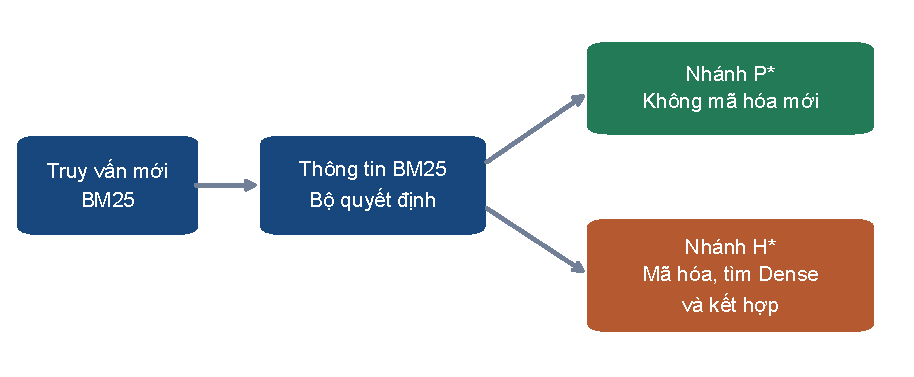
\includegraphics[width=\textwidth]{pegh_principle.pdf}
\caption{Nguyên lý lựa chọn của PE-GH. Bộ quyết định lựa chọn có sử dụng thêm truy xuất ngữ nghĩa trước khi mã hóa truy vấn mới.}
\label{fig:principle}
\end{figure}

Trong hệ thống cuối, nhánh chi phí thấp \Pstar{} sử dụng danh sách BM25 cùng thông tin ngữ nghĩa đã chuẩn bị trước để điều chỉnh thứ tự kết quả. Nhánh này vẫn phát sinh thêm chi phí so với trả trực tiếp BM25, nhưng không cần mã hóa truy vấn mới. Vì vậy, gọi \Pstar{} là nhánh chi phí thấp mang ý nghĩa so sánh với Hybrid, không có nghĩa mọi công việc xử lý sau BM25 đều được loại bỏ.

Nhánh \Hstar{} sử dụng thêm Dense rồi kết hợp với kết quả BM25. Mô hình ngữ nghĩa và cách kết hợp được lựa chọn trong giai đoạn phát triển, sau đó giữ cố định khi đánh giá sáu miền xác nhận. Các bộ quyết định trong phép so sánh cùng sử dụng hai nhánh này. Điều kiện đó giúp làm rõ ảnh hưởng của việc chọn truy vấn, thay vì để khác biệt về chất lượng nhánh truy xuất chi phối kết luận.

Đặt quyết định ở vị trí này có một hệ quả trực tiếp: truy vấn bị bỏ qua Dense tránh được cả mã hóa truy vấn và tìm kiếm vector. Tuy nhiên, truy vấn được chuyển sang \Hstar{} vẫn phải trả chi phí BM25, bộ quyết định và nhánh Dense. Do đó, phần tiết kiệm kỳ vọng xuất hiện nhờ một tỷ lệ truy vấn kết thúc ở nhánh rẻ. Nếu tỷ lệ đó quá nhỏ hoặc nhánh rẻ quá tốn kém, hiệu quả đầu cuối có thể hạn chế dù lựa chọn không làm giảm nhiều chất lượng.

\section{Thông tin dùng cho quyết định}
Bộ quyết định v2 sử dụng thông tin về nội dung truy vấn, mức độ phù hợp của từ ngữ với kho câu hỏi và biểu hiện của danh sách BM25. Những thông tin này đều có sẵn trước khi chạy Dense. Ràng buộc đó là điều kiện để PE-GH có thể lựa chọn sử dụng truy xuất ngữ nghĩa trước khi phát sinh chi phí của nhánh này.

\begin{table}[htbp]
\centering\small
\caption{Nhóm thông tin dùng cho bộ quyết định và ý nghĩa đối với bài toán.}
\label{tab:features}
\begin{tabularx}{\textwidth}{@{}p{32mm}YY@{}}
\hline
\textbf{Nhóm thông tin} & \textbf{Ví dụ tín hiệu} & \textbf{Câu hỏi mà tín hiệu hỗ trợ}\\\hline
Đặc điểm truy vấn & Cách diễn đạt và mức độ cụ thể của từ ngữ. & Truy vấn chứa những dấu hiệu nào về nhu cầu tìm kiếm?\\
Quan hệ với kho câu hỏi & Mức độ xuất hiện của từ ngữ truy vấn trong dữ liệu. & Kho câu hỏi có bao phủ cách diễn đạt của truy vấn hay không?\\
Danh sách BM25 & Mức nổi bật của các kết quả đầu và sự khác biệt giữa chúng. & Kết quả từ khóa có tạo ra bằng chứng rõ về mức độ liên quan hay không?\\
Dự báo chất lượng & Các dấu hiệu về mức độ chắc chắn của kết quả từ khóa. & Truy vấn có nguy cơ không được BM25 đáp ứng hay không?\\
\hline
\end{tabularx}
\end{table}

Các nhóm trong Bảng~\ref{tab:features} không được diễn giải thành quy luật chắc chắn cho từng truy vấn. Chẳng hạn, khoảng cách điểm lớn có thể biểu thị một kết quả nổi bật, nhưng kết quả nổi bật vẫn có thể không liên quan. Bộ quyết định học mối liên hệ thống kê giữa những tín hiệu này và nhãn BM25 thất bại trên dữ liệu phát triển. Vì thế, ý nghĩa của một đặc trưng nằm trong tổ hợp thông tin và phạm vi đã học, không phải ở một điều kiện đơn lẻ luôn đúng.

Mức phổ biến từ ngữ và đặc điểm kết quả tìm kiếm khác nhau giữa các miền. Khi áp dụng ở miền xác nhận, hệ thống được tiếp cận một tập truy vấn không có nhãn để thích nghi với khác biệt đó, nhưng không học lại bộ quyết định bằng nhãn liên quan của miền này. Do đó, kết quả chuyển miền cần được hiểu trong điều kiện có sẵn truy vấn đại diện. Báo cáo không xem đây là bằng chứng cho trường hợp triển khai ngay ở một miền hoàn toàn chưa có dữ liệu.

Việc sử dụng nhiều thông tin hơn cần được đánh giá bằng đóng góp thực tế đối với chất lượng lựa chọn. Một bộ quyết định phức tạp hơn chưa chắc giúp tìm được câu hỏi phù hợp hơn. Các phân tích ở chương kết quả vì thế tập trung vào hiệu quả cuối cùng, đồng thời xem xét liệu thay đổi mục tiêu dự báo có phù hợp với thông tin mà hệ thống đang quan sát hay không.

\section{Cơ sở lựa chọn cách học cho bộ quyết định}
Phiên bản đầu của PE-GH dự đoán lợi ích khi thay BM25 bằng Hybrid. Nhãn này gần mục tiêu hành động, nhưng phụ thuộc kết quả của cả hai nhánh, trong khi bộ quyết định chỉ quan sát phía BM25. Khi Dense yếu hoặc phản ứng của encoder không được các đặc trưng từ khóa phản ánh tốt, bài toán dự đoán lợi ích có thể khó hơn kỳ vọng. Các vòng đầu chưa cho bằng chứng đủ mạnh rằng mô hình học theo hướng đó vượt quy tắc margin ở cùng ngân sách.

Hệ thống v2 chuyển sang nhận biết trường hợp BM25 không tìm được tài liệu liên quan trong mười kết quả đầu. Bộ quyết định học từ những truy vấn đã có nhãn để ưu tiên sử dụng thêm Dense khi xuất hiện dấu hiệu của tình huống này. Mục tiêu dự báo gắn trực tiếp với chất lượng của danh sách BM25 mà hệ thống quan sát được, nên phù hợp hơn với nguồn thông tin có sẵn trước khi chạy Dense.

Lý do dùng bộ quyết định nhẹ xuất phát từ chính mục tiêu tiết kiệm. Nếu việc lựa chọn tốn gần bằng phần truy xuất có thể bỏ qua, hệ thống khó thu được lợi ích về thời gian xử lý. Vì vậy, PE-GH ưu tiên một cách dự báo có chi phí thấp, đủ để sắp thứ tự truy vấn theo mức cần hỗ trợ. Giá trị của lựa chọn này được kiểm tra bằng cả chất lượng danh sách cuối và chi phí phục vụ thực tế.

Việc huấn luyện gộp sáu miền hướng đến nhận biết tín hiệu vượt ra ngoài một chủ đề cụ thể. Trong phát triển, mỗi miền được lần lượt để riêng để kiểm tra mô hình học trên các miền còn lại. Sau khi lựa chọn cấu hình, bộ quyết định được học trên cả sáu miền phát triển rồi đóng băng. Quy trình này giảm yêu cầu phải có nhãn của từng miền xác nhận, đồng thời cho phép đánh giá một mô hình cố định trong phạm vi rộng hơn bản đầu.

Tuy vậy, nhận biết BM25 thất bại chưa đồng nghĩa nhận biết đúng truy vấn được Hybrid cải thiện nhiều nhất. Dense cũng có thể không tìm được kết quả phù hợp cho một truy vấn khó, còn truy vấn đã có kết quả từ khóa liên quan vẫn có thể hưởng lợi từ Hybrid. Vì vậy, báo cáo sử dụng thêm một đối chứng biết trước chất lượng của cả hai nhánh để chỉ ra khoảng cách giữa lựa chọn hiện tại và lựa chọn lý tưởng.

Sự thay đổi đồng thời về nhãn, dữ liệu huấn luyện, encoder và nhánh truy xuất cũng giới hạn cách giải thích tiến bộ giữa hai phiên bản. Kết quả v2 tốt hơn v1 có thể cho thấy hệ thống cuối phù hợp hơn, nhưng không đủ để tách riêng tác động của từng lựa chọn. Những nhận định về nguyên nhân chỉ được đưa ra theo mức bằng chứng mà các thí nghiệm đối chứng thực sự hỗ trợ.

\section{Vai trò của ngân sách truy xuất}
Ngân sách giúp thể hiện mục tiêu sử dụng Dense một cách trực tiếp. Với ngân sách thấp, hệ thống ưu tiên một phần nhỏ truy vấn có điểm quyết định cao. Với ngân sách cao, nhiều truy vấn được chuyển sang Hybrid hơn, nên chất lượng thường tiến gần mốc luôn chạy Hybrid trong các kết quả quan sát. Mối liên hệ này cần được xem bằng đường cong thay vì giả định điểm quyết định tương ứng với một mức tiết kiệm thời gian cố định.

Trong so sánh cùng ngân sách, các bộ quyết định được cấp cùng số lượt Dense trên mỗi phần dữ liệu đánh giá. Chúng lựa chọn bằng điểm dự báo, không dùng nhãn liên quan của truy vấn đang được đánh giá. Kết quả vì thế cho biết phương pháp nào ưu tiên truy vấn hữu ích hơn khi có cùng mức tài nguyên. Tuy nhiên, phép so sánh trên một tập truy vấn đã xác định chưa bảo đảm hệ thống phục vụ liên tiếp sẽ luôn đạt đúng tỷ lệ đó.

Ở điểm vận hành, chính sách lựa chọn được xác định từ những truy vấn chưa có nhãn và giữ cố định trong khi đánh giá. Nếu đặc điểm truy vấn thay đổi, tỷ lệ thực tế sử dụng Dense có thể lệch khỏi ngân sách dự kiến. Những truy vấn mà BM25 không cung cấp được tín hiệu từ khóa cũng cần được chuyển sang Dense. Vì vậy, ngân sách là mục tiêu phân bổ tài nguyên, còn tỷ lệ quan sát phải được báo cáo cùng chất lượng và thời gian xử lý.

Ngân sách vận hành 80\% được chọn trong giai đoạn phát triển theo mục tiêu giảm số lượt Dense mà vẫn giữ chất lượng gần Hybrid. Tiêu chí lựa chọn khi đó chỉ chấp nhận mức giảm không quá 0,005. Sau khi chốt điểm vận hành, giai đoạn xác nhận sử dụng biên suy giảm 0,01 để kiểm tra trên các miền khác. Hai giá trị phục vụ hai vai trò khác nhau: một giá trị dùng để chọn phương án, còn giá trị kia dùng để kết luận trên dữ liệu xác nhận.

\section{Quá trình hình thành phương pháp cuối}
\begin{table}[htbp]
\centering\small
\caption{Các bước phát triển dẫn đến PE-GH v2.}
\label{tab:versions}
\begin{tabularx}{\textwidth}{@{}p{24mm}YY@{}}
\hline
\textbf{Giai đoạn} & \textbf{Cách tiếp cận chính} & \textbf{Bài học cho hệ thống cuối}\\\hline
PE-GH v1 & Dự đoán lợi ích Hybrid từ dữ liệu của từng miền. & Có thể giảm chi phí, nhưng chưa cho thấy lựa chọn tốt hơn margin khi cùng ngân sách.\\
Vòng v3 & Xem xét các phương án truy xuất có chi phí thấp hơn. & Cần giữ đối chứng từ khóa mạnh và kiểm tra quan hệ giữa tín hiệu BM25 với lợi ích Dense.\\
PE-GH v2 trong vòng v4 & Dự báo BM25 thất bại và học từ nhiều miền. & Xác nhận phương pháp đã chốt trên sáu miền chưa dùng để lựa chọn.\\
\hline
\end{tabularx}
\source{Tổng hợp từ các vòng thực nghiệm của nhóm}
\end{table}

Quá trình ở Bảng~\ref{tab:versions} cho thấy kết quả chưa đạt kỳ vọng có vai trò trong việc thu hẹp câu hỏi nghiên cứu. Vấn đề không còn là xây một bộ quyết định bất kỳ để bỏ qua Dense, mà là tìm một cách học phù hợp với thông tin sẵn có và kiểm chứng nó trước một quy tắc đơn giản. Những phương án tiết kiệm khác cũng được giữ trong đánh giá để xác định lựa chọn truy vấn có giá trị ở điều kiện nào.

Hệ thống cuối giữ cấu trúc quyết định trước encoder nhưng thay đổi những yếu tố ảnh hưởng trực tiếp đến chất lượng hai nhánh và khả năng dự báo. Báo cáo vì vậy đánh giá cả hệ thống và khả năng lựa chọn trong cùng một khung đối chứng. Chương tiếp theo mô tả cách tổ chức dữ liệu và phép so sánh để các kết luận về hai mức này không bị trộn lẫn.
